\documentclass[tikz,border=6pt]{standalone}
\usepackage{amsmath}
\usetikzlibrary{arrows.meta,positioning}
\usepackage[dvipsnames]{xcolor}

\begin{document}
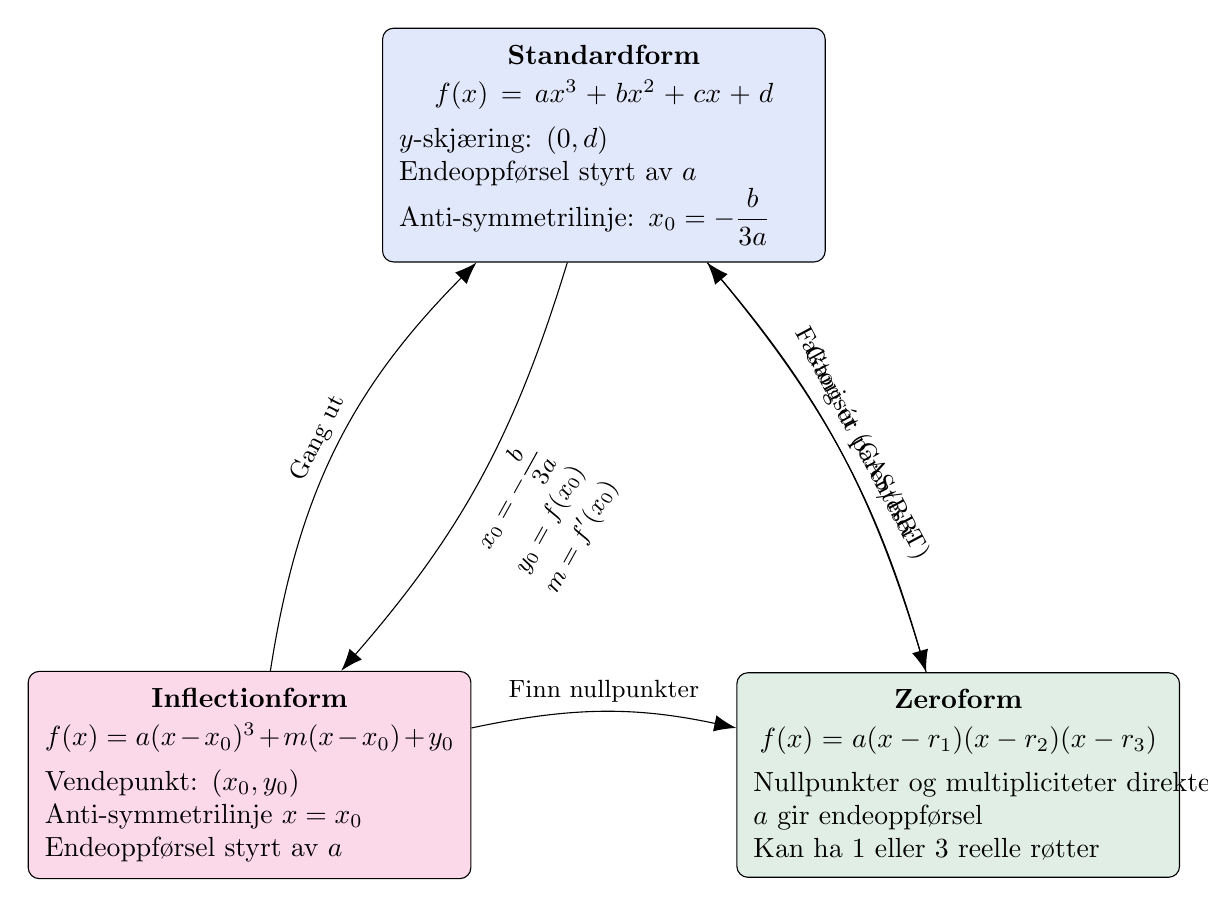
\begin{tikzpicture}[
  >={Latex[length=2.8mm]},
  box/.style   = {
    draw, rounded corners,
    align=center,
    inner sep=6pt,
    minimum width=\boxw,
    text width=\boxw,   % prevent width from growing
    fill=black!3
  },
  label/.style = {font=\small, align=center}
]

% ---- constants ----
\def\L{9}            % triangle side length
\def\H{8}            % height ~ (sqrt3/2)*L
\def\boxw{52mm}      % fixed width for every box

% ---- nodes (equilateral triangle) ----
\node[box, fill=RoyalBlue!15] (std) at (0,\H) {
  \textbf{Standardform}\\[2pt]
  $f(x)=ax^3+bx^2+cx+d$\\[4pt]
  \makebox[\boxw][l]{\normalsize $y$-skjæring: $(0,d)$}\\
  \makebox[\boxw][l]{\normalsize Endeoppførsel styrt av $a$}\\
  \makebox[\boxw][l]{\normalsize Anti-symmetrilinje: $x_0=-\dfrac{b}{3a}$}
};

\node[box, fill=RubineRed!15] (ext) at (-\L/2,0) {
  \textbf{Inflectionform}\\[2pt]
  $f(x)=a(x-x_0)^3+m(x-x_0)+y_0$\\[4pt]
  \makebox[\boxw][l]{\normalsize Vendepunkt: $(x_0,y_0)$}\\
  \makebox[\boxw][l]{\normalsize Anti-symmetrilinje $x = x_0$}\\
  \makebox[\boxw][l]{\normalsize Endeoppførsel styrt av $a$}\\
};

\node[box, fill=SeaGreen!15] (nul) at (\L/2,0) {
  \textbf{Zeroform}\\[2pt]
  $f(x)=a(x-r_1)(x-r_2)(x-r_3)$\\[4pt]
  \makebox[\boxw][l]{\normalsize Nullpunkter og multipliciteter direkte}\\
  \makebox[\boxw][l]{\normalsize $a$ gir endeoppførsel}\\
  \makebox[\boxw][l]{\normalsize Kan ha 1 eller 3 reelle røtter}
};

% ---- arrows (circular-style bends) ----
% Standard -> Inflection
\draw[->] (std) to[bend left=12]
  node[label,midway,sloped,below] {$x_0=-\dfrac{b}{3a}$\\[2pt] $y_0=f(x_0)$\\[2pt] $m=f'(x_0)$}
  (ext);

% Inflection -> Zero
\draw[->] (ext) to[bend left=12]
  node[label,midway,sloped,above] {Finn nullpunkter}
  (nul);

% Zero -> Standard
\draw[->] (nul) to[bend right=12]
  node[label,midway,sloped,above] {Gang ut parenteser}
  (std);

% Inflection -> Standard
\draw[->] (ext) to[bend left=18]
  node[label,midway,sloped,above] {Gang ut}
  (std);

% Standard -> Zero (factor)
\draw[->] (std) to[bend left=12]
  node[label,midway,sloped,above] {Faktorisér (CAS/RRT)}
  (nul);

\end{tikzpicture}
\end{document}